\subsection{Reading Edgelist from text file}

We attempt a number of approaches to read edgelist from text file into in-memory edgelist(s), given in Sections \ref{sec:el-fstream-plain}-\ref{sec:el-mmap-custom}. Among these, we find using \texttt{mmap()} with custom number parsers (\textit{mmap-custom}) to be the best approach. The pseudocode for \textit{mmap-custom} is given Algorithm \ref{alg:el}.

\begin{algorithm}[hbtp]
\caption{Reading Edge-list from file.}
\label{alg:el}
\begin{algorithmic}[1]
\Require{$pdegrees$: Per partition vertex degrees (output)}
\Require{$edges$: Per thread sources, targets, and weights of edges (output)}
\Require{$data$: Memory mapped file data}
\Ensure{$counts$: Number of edges read per thread (output)}
\Ensure{$symmetric$: Is graph symmetric?}
\Ensure{$weighted$: Is graph weighted?}
\Ensure{$\beta$: Size of each block that is processed per thread}
\Ensure{$\rho$: Number of partitions for counting vertex degrees}
\Ensure{$t$: Current thread}

\Statex

\Function{getBlock}{$data, i$} \label{alg:frontier--main-begin}
  \State $[d, D] \gets data$
  \State $b \gets d+i$ \textbf{;} $B \gets min(b+\beta, D)$
  \If{$b \neq d$ \textbf{and not} $isNewline(b-1)$}
    \State $b \gets findNextLine(b, D)$
  \EndIf
  \If{$B \neq d$ \textbf{and not} $isNewline(B-1)$}
    \State $B \gets findNextLine(B, D)$
  \EndIf
  \Return{$[b, B]$}
\EndFunction

\Statex
  
\Function{readEdgelist}{$pdegrees, edges, data$}
  \State $counts \gets \{0\}$
  \State $[sources, targets, weights] \gets edges$
  \State $\rhd$ Load edges from text file in blocks of size $\beta$
  \ForAll{$i \in [0, \beta, 2\beta, ... |data|]$ \textbf{in parallel}}
    \State $j \gets counts[t]$
    \State $[b, B] \gets getBlock(data, i)$
    \While{$true$}
      \State $\rhd$ Read an edge from the block
      \State $u \gets v \gets 0$ \textbf{;} $w \gets 1$
      \State $b \gets findNextDigit(b, B)$
      \If{$b = B$} \textbf{break}
      \EndIf
      \State $b \gets parseWholeNumber(u, b, B)$
      \State $b \gets findNextDigit(b, B)$
      \State $b \gets parseWholeNumber(v, b, B)$
      \If{$weighted$}
        \State $b \gets findNextDigit(b, B)$
        \State $b \gets parseFloat(w, b, B)$
      \EndIf
      \State $\rhd$ Make it zero-based
      \State $u \gets u - 1$ \textbf{;} $v \gets v - 1$
      \State $\rhd$ Add the parsed edge to edgelist
      \State $sources[t][j] \gets u$
      \State $targets[t][j] \gets v$
      \If{$weighted$} $weights[t][j] \gets w$
      \EndIf
      \State $atomicAdd(pdegrees[t \bmod \rho][u], 1)$
      \State $j \gets j + 1$
      \State $\rhd$ If graph is symmetric, add the reverse edge
      \If{$symmetric$}
        \State $sources[t][j] \gets v$
        \State $targets[t][j] \gets u$
        \If{$weighted$} $weights[t][j] \gets w$
        \EndIf
        \State $atomicAdd(pdegrees[t \bmod \rho][v], 1)$
        \State $j \gets j + 1$
      \EndIf
    \EndWhile
    \State $counts[t] \gets j$
  \EndFor
  \Return{$counts$}
\EndFunction
\end{algorithmic}
\end{algorithm}



\subsubsection{\texttt{ifstream} with \texttt{getline()} and \texttt{>>} operator (\textit{fstream-plain})}
\label{sec:el-fstream-plain}

In this approach, we utilize C++'s \texttt{ifstream} to open the file, and read the edges line by line with \texttt{getline()}. If the graph is unweighted, we read the source and target vertex ids as 64-bit unsigned integers, using \texttt{>>} operator, into pre-allocated source and target arrays based on information in the file header. If the graph is weighted, we also read the weights as 32-bit floating-point numbers into another pre-allocated array. This process is sequential, given that streams are inherently sequential.


\subsubsection{\texttt{ifstream} with \texttt{getline()} and \texttt{strto*()} (\textit{fstream-strto*})}
\label{sec:el-fstream-stro*}

In this approach, we again use \texttt{ifstream} but employ string-to-number conversion methods \texttt{strtoull()} and \texttt{strtod()} for parallel number parsing. We sequentially read a block of $L$ lines from the file, using \texttt{getline()}, and then parse each line in parallel using multiple threads. We observe that using OpenMP's dynamic scheduling, with a chunk size of $1024$, and reading a block of $L=128K$ lines to be processed in parallel offers the best performance. Parsed edges (source, target vertex ids, and edge weights) are stored separately in per-thread edge lists to avoid contention issues within a shared data structure. With 64 threads, this approach demonstrates a speedup of XX compared to \textit{fstream-plain}, as shown in Figure \ref{fig:optimize-el}.


\subsubsection{\texttt{fopen()} with \texttt{fgets()} and \texttt{sscanf()} (\textit{fopen-plain})}
\label{sec:el-fopen-plain}

This approach is similar to the one mentioned above (\textit{fscanf-strto*}), but we use \texttt{fgets()} on a file handle to read lines instead of \texttt{getline()}, and employ \texttt{sscanf()} to parse the edges. With 64 threads, it provided a speedup of X compared to X.


\subsubsection{\texttt{fopen()} with \texttt{fgets()} and \texttt{strto*()} (\textit{fopen-strto*})}
\label{sec:el-fopen-strto*}

Similar to the previous approach (\textit{fopen-plain}), this one uses \texttt{fgets()} to read lines from the text file, but replaces \texttt{sscanf()} with \texttt{strtoull()} and \texttt{strtod()}. This proves faster due to the absence of a format string. With 64 threads, it provides a speedup of X over X.


\subsubsection{\texttt{mmap()} with \texttt{strto*()} (\textit{mmap-strto*})}
\label{sec:el-mmap-strto*}

In this approach, we map the file to memory with \texttt{mmap()}, and process the edges in parallel by partitioning the file into blocks of $C$ characters. Each block is dynamically assigned (using OpenMP's dynamic schedule) to a free thread. If the assigned block contains partial lines at either end, the thread repositions it, by shifting to the right to eliminate partial lines. This involves skipping the partial line at the beginning and including the partial line from the end. We observe that issuing \texttt{madvice(MADV\_WILLNEED)}, and using a block size of $C=256K$ characters offers the best performance. To parse the source/target vertex ids and edge weights, we use \texttt{strtoull()} and \texttt{strtod()}. Each thread stores the parsed edges in per-thread edgelists.


\subsubsection{\texttt{mmap()} with custom number parsers (\textit{mmap-custom})}
\label{sec:el-mmap-custom}

This is similar to the approach mentioned above (\textit{mmap-strto*}), but we use our own functions for parsing whole numbers and floating-point numbers. In addition, as vertex ids start with $1$, we decrement $1$ from the vertex ids after parsing it and before appending them to per-thread edgelists. Surprisingly, this leads to $40-50\%$ drop in performance. Converting the $weighted$ flag (see Algorithm \ref{alg:el}) to a template parameter solves this issue. This indicates that the issue was related to the loop code not being able to fit in the code cache of the processor and using a template allowed it to fit in the cache. Accordingly, we also recommend using $symmetric$ flag to be used as a template parameter instead. With 64 threads, it provides a speedup of X over X, as show in Figure \ref{fig:optimize-el}. We also attempted to use custom SIMD instructions to parse numbers, along with \texttt{vzeroupper} instruction to clear SSE/AVX registers, but it did not provide additional performance improvement.


\subsubsection{Explanation of \textit{mmap-custom} approach (Algorithm \ref{alg:el})}

We now explain the psuedocode of \textit{mmap-custom} approach, which loads per-thread edgelists from a file with the best performance. Consider the \texttt{readEdgelist()} function. In Lines X-X various variables are initialized, including the counts of edges read per thread ($counts$), arrays for sources, targets, and weights ($edges$), and other parameters. This is followed by a loop (Lines X-X), where each iteration processes a block of characters in the text file in parallel across different threads. The loop iterates over block of $data$, starting from index $i$ with a step size of $\beta = 256K$. Inside the loop, $j$ keeps track of the number of edges processed by the current thread. In Line X, the \texttt{getBlock()} function is called to retrieve the current block of data ($[b, B]$). The algorithm then enters a While loop to read edges from the block in Line X-X. Edge information (source, target, weight) is parsed from the block, and, if the graph is weighted, the weight is also parsed. In Line X-X, Parsed edges are adjusted to be zero-based, and vertex degrees are updated in the pdegrees array. Then, in Lines X-X, the parsed edges are added to the arrays (sources, targets, weights) for the current thread. If the graph is symmetric, reverse edges are added as well. The loop continues until the entire block is processed, updating j and counting the number of edges processed by the current thread. Finally, the number of edges read by each thread are returned.

The \texttt{getBlock()} function (Lines X-X) retrieves a block of characters to process from the memory-mapped file, starting from index $i$. It ensures that the block starts and ends on newline characters for proper parsing. The block size is determined by the parameter $\beta$, which is set to $256K$.

\begin{figure}[hbtp]
  \centering
  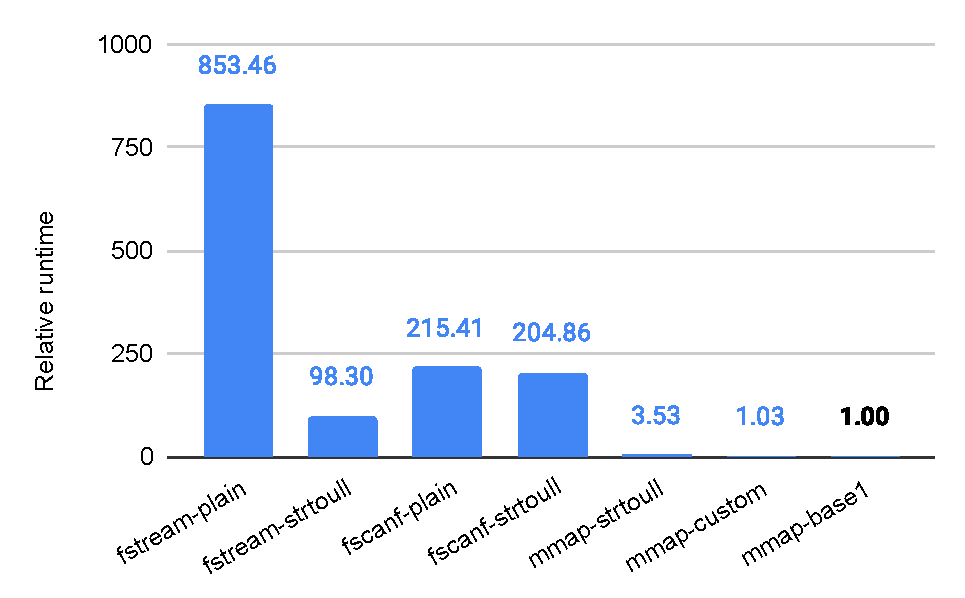
\includegraphics[width=0.99\linewidth]{out/optimize-el.pdf} \\[-2ex]
  \caption{Gini coefficient of PageRank values on 24 different graphs, comparing between PageRank values obtained with three different dead-end handling strategies: \textit{teleport from dead-ends} (\textbf{default}), \textit{self-loop dead-ends} (\textbf{loop}), and \textit{self-loop all vertices} (\textbf{loopall}).}
  \label{fig:optimize-el}
\end{figure}




\subsection{Converting Edgelist to CSR}

\begin{algorithm}[hbtp]
\caption{Convert Edge-list to CSR.}
\label{alg:csr}
\begin{algorithmic}[1]
\Require{$csr$: Global CSR (output)}
\Require{$pcsr$: Per partition CSR (scratch)}
\Require{$pdegrees$: Per partition vertex degrees (scratch)}
\Require{$edges$: Per thread sources, targets, and weights of edges}
\Require{$counts$: Number of edges read per thread}
\Ensure{$symmetric$: Is graph symmetric?}
\Ensure{$weighted$: Is graph weighted?}
\Ensure{$\rho$: Number of partitions for counting vertex degrees}
\Ensure{$t$: Current thread}

\Statex

\Function{convertToCsr}{$csr, pcsr, pdegrees, edges, counts$}
  \State $[offsets, edgeKeys, edgeValues] \gets csr$ \label{alg:csr--initialize-begin}
  \State $[poffsets, pedgeKeys, pedgeValues] \gets pcsr$
  \State $[sources, targets, weights] \gets edges$ \label{alg:csr--initialize-end}
  \State $\rhd$ Compute offsets
  \ForAll{$p \in [0, \rho)$} \label{alg:csr--poffsets-begin}
    \State $exclusiveScan(poffsets[p], pdegrees[p], |V|+1)$
  \EndFor \label{alg:csr--poffsets-end}
  \State $\rhd$ Populate per-partition CSR
  \ForAll{\textbf{threads in parallel}} \label{alg:csr--pcsr-begin}
    \ForAll{$i \in [0, counts[t])$}
      \State $u \gets sources[t][i]$
      \State $v \gets targets[t][i]$
      \State $j \gets atomicAdd(poffsets[t \bmod \rho][u], 1)$
      \State $pedgeKeys[t \bmod \rho][j] \gets v$
      \If{$weighted$}
        \State $pedgeValues[t \bmod \rho][j] \gets weights[t][i]$
      \EndIf
    \EndFor
  \EndFor \label{alg:csr--pcsr-end}
  \State $\rhd$ Fix per-partition offsets
  \ForAll{\textbf{threads in parallel}} \label{alg:csr--poffsets-fix-begin}
    \If{$t < \rho$}
      \State $memcpy(poffsets[t]+1, poffsets[t], |V|)$
      \State $poffsets[t][0] \gets 0$
    \EndIf
  \EndFor \label{alg:csr--poffsets-fix-end}
  \State $\rhd$ Combine per-partition degrees
  \ForAll{$u \in [0, |V|)$ \textbf{in parallel}} \label{alg:csr--poffsets-combine-begin}
    \ForAll{$p \in [1, \rho)$}
      \State $pdegrees[0][u] +\gets pdegrees[p][u]$
    \EndFor
  \EndFor \label{alg:csr--poffsets-combine-end}
  \State $\rhd$ Compute global offsets
  \State $exclusiveScan(offsets, pdegrees[0], |V|+1)$ \label{alg:csr--offsets-compute}
  \State $\rhd$ Combine per-partition CSR into one CSR
  \ForAll{$u \in [0, |V|)$ \textbf{in parallel}} \label{alg:csr--pcsr-combine-begin}
    \State $j \gets offsets[u]$
    \ForAll{$p \in [0, \rho)$}
      \State $i \gets poffsets[t][u]$
      \State $I \gets poffsets[t][u+1]$
      \ForAll{$i \in [i, I)$}
        \State $edgeKeys[j] \gets pedgeKeys[t][i]$
        \If{$weighted$}
          \State $edgeValues[j] \gets pedgeValues[t][i]$
        \EndIf
        \State $j \gets j + 1$
      \EndFor
    \EndFor
  \EndFor \label{alg:csr--pcsr-combine-end}
\EndFunction
\end{algorithmic}
\end{algorithm}



\subsubsection{Obtain global vertex degrees along with reading Edgelist (\textit{degree-global})}

Now that we have obtained per-thread edgelists, we must now convert the edgelists to CSR. To do this, we first need to know the degree of each vertex. In this approach, A simple solution for this is to update the degree of each vertex in a common array, using atomic operations, while reading the edgelists. The relative runtime of this approach with respect to simple reading per-thread edgelists is XX, as shown in Figure \ref{fig:optimize-csr}. We however observe that this results in high contention and impacts performance.


\subsubsection{Obtain per-thread vertex degrees along with reading Edgelist (\textit{degree-thread})}

In this approach, we compute per-thread vertex degrees instead of global degrees. While this improves performance by X\% compared to obtaining global vertex degrees, it requires significant additional space, and needs to be combined later to obtain global degrees. We observe that computing degrees in partitions of $4$ (using $\bmod 4$) and then combining them gives us the best performance.


\subsubsection{Obtain CSR from global vertex degrees (\textit{csr-global})}

Now that we have the degrees, we need to combine the per-thread edgelists into a CSR data structure. In this approach, we first obtain global vertex degrees along with read per-thread edgelists (as with \textit{degree-global}), and the convert the per-thread edgelists to a global CSR in parallel using atomic operations. However, this approach has poor performance.


\subsubsection{Obtain CSR from 4-partitioned vertex degrees (\textit{csr-partition4})}

Next, we explore computing CSR in k partitions and later combining them. Our observations indicate that using 4 partitions to generate CSR and then combining them has the best performance.

Now describe the figures and the algorithm.

\begin{figure}[hbtp]
  \centering
  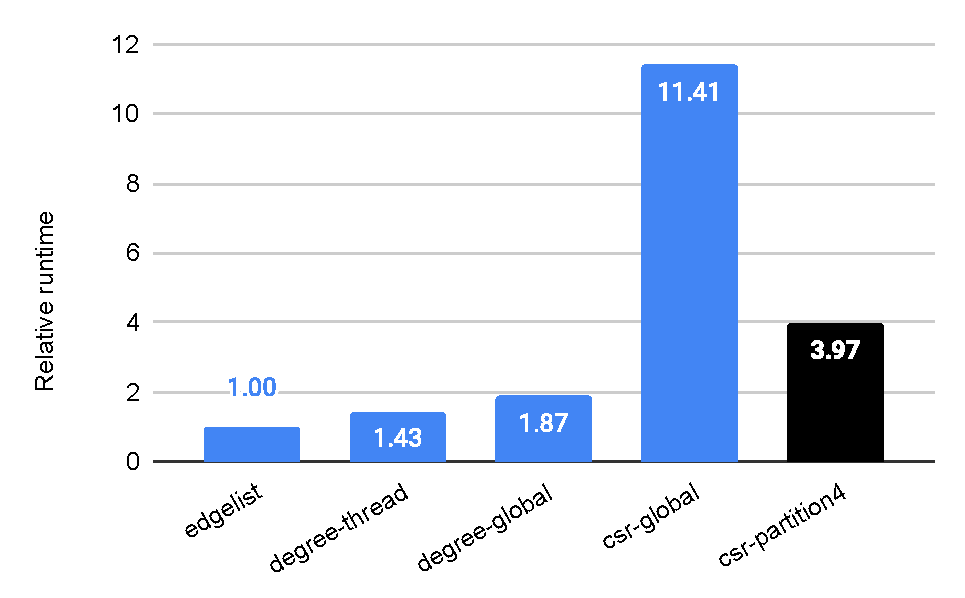
\includegraphics[width=0.99\linewidth]{out/optimize-csr.pdf} \\[-2ex]
  \caption{Gini coefficient of PageRank values on 24 different graphs, comparing between PageRank values obtained with three different dead-end handling strategies: \textit{teleport from dead-ends} (\textbf{default}), \textit{self-loop dead-ends} (\textbf{loop}), and \textit{self-loop all vertices} (\textbf{loopall}).}
  \label{fig:optimize-csr}
\end{figure}

